\documentclass[crop=false,class=article,oneside]{standalone}
%----------------------------Preamble-------------------------------%
%---------------------------Packages----------------------------%
\usepackage{geometry}
\geometry{b5paper, margin=1.0in}
\usepackage[T1]{fontenc}
\usepackage{graphicx, float}            % Graphics/Images.
\usepackage{natbib}                     % For bibliographies.
\bibliographystyle{agsm}                % Bibliography style.
\usepackage[french, english]{babel}     % Language typesetting.
\usepackage[dvipsnames]{xcolor}         % Color names.
\usepackage{listings, lstlinebgrd}      % Verbatim-Like Tools.
\usepackage{mathtools, esint, mathrsfs} % amsmath and integrals.
\usepackage{amsthm, amsfonts}           % Fonts and theorems.
\usepackage{tabularx}
\usepackage{tcolorbox}                  % Frames around theorems.
\usepackage{upgreek}                    % Non-Italic Greek.
\usepackage{paracol}                    % Two-column styling.
\usepackage{wrapfig}                    % Wrap text around figure.
\usepackage{fmtcount, etoolbox}         % For the \book{} command.
\usepackage[newparttoc]{titlesec}       % Formatting chapter, etc.
\usepackage{titletoc}                   % Allows \book in toc.
\usepackage[nottoc]{tocbibind}          % Bibliography in toc.
\usepackage[titles]{tocloft}            % ToC formatting.
\usepackage{multicol, enumitem}         % Multi-column/enumerate.
\usepackage{import}                     % Import external files.
\usepackage{pgfplots, tikz}             % Drawing/graphing tools.
\usetikzlibrary{
    calc,                   % Calculating right angles and more.
    angles,                 % Drawing angles within triangles.
    arrows.meta,            % Latex and Stealth arrows.
    quotes,                 % Adding labels to angles.
    positioning,            % Relative positioning of nodes.
    decorations.markings,   % Adding arrows in the middle of a line.
    patterns,
    arrows,
    shapes,
    shapes.geometric,
    cd,
    hobby,
    babel
}                                       % Libraries for tikz.
\pgfplotsset{compat=1.9}                % Version of pgfplots.
\usepackage[font=scriptsize,
            labelformat=simple,
            labelsep=colon]{subcaption} % Subfigure captions.
\usepackage[font={scriptsize},
            hypcap=true,
            labelsep=colon]{caption}    % Figure captions.
\usepackage{hyperref}                   % Allows for hyperlinks.
\hypersetup{
    colorlinks=true,
    linkcolor=blue,
    filecolor=magenta,
    urlcolor=Cerulean,
    citecolor=SkyBlue
}                           % Colors for hyperref.
\usepackage[toc,acronym,nogroupskip]{glossaries} % Glossaries and acronyms.
\usepackage[subpreambles=false]{standalone}      % Complileable sub files.

% Various font stuff from kiwi.
% Use this for Times text and Computer Modern math
%\usepackage{times}

% Quite nice
%\usepackage[charter, greekfamily=, greekuppercase=italicized]{mathdesign}
%\usepackage[utopia, greekuppercase=italicized]{mathdesign}    % Math is narrower

% Use this for Times text and math
%\usepackage{newtxtext}
%\usepackage[libertine,cmintegrals]{newtxmath}
%\usepackage{fix-cm}

%\usepackage{txfontsb}
% or
%\usepackage{mathptmx}

%\usepackage[scaled=0.92]{helvet}
%\renewcommand{\rmdefault}{ptm}

%\usepackage{mathpazo}    % add possibly `sc` and `osf` options
%\usepackage{eulervm}

%\usepackage{fourier}
%\renewcommand{\rmdefault}{ptm}
%\usepackage{mathptm}

%\usepackage{fontspec}
%\setmainfont{lmodern}

%\usepackage[varg]{txfonts}
%\usepackage{fouriernc}
%\usepackage{mathpazo}

%\usepackage{bookman}
%\usepackage[scaled]{uarial}
%\usepackage[scaled]{helvet}
%\renewcommand*\familydefault{\sfdefault}
%\usepackage[math]{anttor}

%\newcommand\fgeorgia{\fontfamily{jvn}\selectfont}
%\newcommand\ftimes{\fontfamily{ptm}\selectfont}
%\newcommand\fhelvetica{\fontfamily{phv}\selectfont}
%\newcommand\fcourier{\fontfamily{pcr}\selectfont}
%\newcommand\fbookman{\fontfamily{pbk}\selectfont}
%\newcommand\fnewcentury{\fontfamily{pnc}\selectfont}
%\newcommand\fpalatino{\fontfamily{ppl}\selectfont}
%\newcommand\favantgarde{\fontfamily{pag}\selectfont}
%\newcommand\fnormal{\normalfont}
%\newcommand\fsize[1]{\ifnum#1>0\fontsize{#1}{#1}\selectfont\else\normalsize\fi}
%------------------------Theorem Styles-------------------------%
% Define theorem style for default spacing and normal font.
\newtheoremstyle{normal}
    {\topsep}               % Amount of space above the theorem.
    {\topsep}               % Amount of space below the theorem.
    {}                      % Font used for body of theorem.
    {}                      % Measure of space to indent.
    {\bfseries}             % Font of the header of the theorem.
    {}                      % Punctuation between head and body.
    {.5em}                  % Space after theorem head.
    {}

% Define theorem style for default spacing with italicized font.
\newtheoremstyle{normalit}{\topsep}{\topsep}
                {\itshape}{}{\bfseries}{}{.5em}{}

% Italic header environment.
\newtheoremstyle{thmit}{\topsep}{\topsep}{}{}{\itshape}{}{0.5em}{}

% Define italicized environments.
\theoremstyle{normalit}
\newtheorem{theorem}{Theorem}[section]
\newtheorem{lemma}{Lemma}[section]
\newtheorem{corollary}{Corollary}[section]
\newtheorem{proposition}{Proposition}[section]
\newtheorem*{theorem*}{Theorem}

% Define environments with italic headers.
\theoremstyle{thmit}
\newtheorem*{solution}{Solution}
\newtheorem*{fsolution}{Solution}

% Define default environments.
\theoremstyle{normal}
\newtheorem{example}{Example}[section]
\newtheorem{definition}{Definition}[section]
\newtheorem{problem}{Problem}[section]
\newtheorem{question}{Question}[section]
\newtheorem{remark}{Remark}[section]
\newtheorem{properties}{Properties}[section]
\newtheorem{notation}{Notation}[section]
\newtheorem{axiom}{Axiom}[section]
\newtheorem*{properties*}{Properties}
\newtheorem*{remark*}{Remark}
\newtheorem*{definition*}{Definition}
\theoremstyle{plain}

% Define framed environment.
\tcbuselibrary{most}
\newtcbtheorem[use counter*=theorem]{ftheorem}{Theorem}%
    {colback=green!5,colframe=green!35!black,
     fonttitle=\bfseries\upshape}{th}

\newtcbtheorem[use counter*=example]{fdefinition}{Definition}%
    {fonttitle=\bfseries\upshape,
     colback=blue!5!white,colframe=blue!75!black}{def}

\newtcbtheorem[use counter*=example]{fexample}{Example}%
    {fonttitle=\bfseries\upshape,
     colback=red!5!white,colframe=red!75!black}{ex}

\newtcbtheorem[use counter*=notation]{fnotation}{Notation}%
    {fonttitle=\bfseries\upshape,
     colback=SeaGreen!5!white,colframe=SeaGreen!75!black}{ex}

\newtcbtheorem[use counter*=corollary]{fcorollary}{Corollary}%
    {fonttitle=\bfseries\upshape,
     colback=Orchid!5!white,colframe=Orchid!75!black}{ex}

\newenvironment{bproof}{\textit{Proof.}}{\hfill$\square$}
\tcolorboxenvironment{bproof}{blanker,breakable,left=5mm,
                             before skip=10pt,after skip=10pt,
                             borderline west={1mm}{0pt}{red}}
\tcolorboxenvironment{fsolution}
    {enhanced jigsaw,colframe=cyan,interior hidden,breakable}

%--------------------Declared Math Operators--------------------%
\DeclareMathOperator{\Refl}{Refl}           % Reflection operator.
\DeclareMathOperator{\Span}{Span}           % Span of a set of vectors.
\DeclareMathOperator{\Card}{Card}           % Cardinality of set.
\DeclareMathOperator{\Ord}{Ord}             % Ordinal of ordered set.
\DeclareMathOperator{\Tr}{Tr}               % Trace of matrix.
\DeclareMathOperator{\adjoint}{adj}         % Adjoint of matrix.
\DeclareMathOperator{\rk}{rk}               % Rank of operator.
\DeclareMathOperator{\nul}{nul}             % Null space of operator.
\DeclareMathOperator{\sgn}{sgn}             % Sign of a number.
\DeclareMathOperator{\multideg}{mutlideg}   % Multi-Degree (Graphs).
\DeclareMathOperator{\GCD}{GCD}             % Greatest common denominator.
\DeclareMathOperator{\LM}{LM}               % Leading monomial
\DeclareMathOperator{\LC}{LC}               % Leading coefficient.
\DeclareMathOperator{\LT}{LT}               % Leading term.
\DeclareMathOperator{\LCM}{LCM}             % Least common multiple.
\DeclareMathOperator{\Mon}{Mon}             % Monomial.
\DeclareMathOperator{\Spec}{Spec}           % Spectrum.
\DeclareMathOperator{\proj}{proj}           % Projection.
\DeclareMathOperator{\comp}{comp}           % Component.
\DeclareMathOperator{\sinc}{sinc}           % Sinc function.
\DeclareMathOperator{\Ima}{Im}              % Image of operator.
\DeclareMathOperator{\Prin}{Prin}           % Principal value.
\DeclareMathOperator{\Mod}{mod}             % Modulus.
%------------------------New Commands---------------------------%
\DeclarePairedDelimiter\norm{\lVert}{\rVert}
\DeclarePairedDelimiter\ceil{\lceil}{\rceil}
\DeclarePairedDelimiter\floor{\lfloor}{\rfloor}
\newcommand*\diff{\mathop{}\!\mathrm{d}}
\newcommand*\Diff[1]{\mathop{}\!\mathrm{d^#1}}
\renewcommand{\mod}{\ \Mod}
\renewcommand*{\glstextformat}[1]{\textcolor{RoyalBlue}{#1}}
\renewcommand{\glsnamefont}[1]{\textbf{#1}}
\renewcommand\labelitemii{$\circ$}
\renewcommand\thesubfigure{\arabic{chapter}.\arabic{figure}}
\renewcommand\thesubfigure{%
    \arabic{chapter}.\arabic{figure}.\arabic{subfigure}}
\addto\captionsenglish{\renewcommand{\figurename}{Fig.}}
%------------------------Book Command---------------------------%
\makeatletter
\renewcommand\@pnumwidth{1cm}
\newcounter{book}
\renewcommand\thebook{\@Roman\c@book}
\newcommand\book{%
    \if@openright
        \cleardoublepage
    \else
        \clearpage
    \fi
    \thispagestyle{plain}%
    \if@twocolumn
        \onecolumn
        \@tempswatrue
    \else
        \@tempswafalse
    \fi
    \null\vfil
    \secdef\@book\@sbook
}
\def\@book[#1]#2{%
    \ifnum \c@secnumdepth >-3\relax
        \refstepcounter{book}%
        \addcontentsline{toc}{book}{
            \bookname\ \thebook:\hspace{1em}#1
        }
    \else
        \addcontentsline{toc}{book}{#1}%
    \fi
    \markboth{}{}%
    {\centering
     \interlinepenalty \@M
     \normalfont
     \ifnum \c@secnumdepth >-2\relax
       \huge\bfseries \bookname\nobreakspace\thebook
       \par
       \vskip 20\p@
     \fi
     \Huge \bfseries #2\par}%
    \@endbook}
\def\@sbook#1{%
    {\centering
     \interlinepenalty \@M
     \normalfont
     \Huge \bfseries #1\par}%
    \@endbook}
\def\@endbook{
    \vfil\newpage
        \if@twoside
            \if@openright
                \null
                \thispagestyle{empty}%
                \newpage
            \fi
        \fi
        \if@tempswa
            \twocolumn
        \fi
}
\newcommand*\l@book[2]{%
    \ifnum \c@tocdepth >-2\relax
        \addpenalty{-\@highpenalty}%
        \addvspace{2.25em \@plus\p@}%
        \setlength\@tempdima{3em}%
        \begingroup
            \parindent \z@ \rightskip \@pnumwidth
            \parfillskip -\@pnumwidth
            {
                \leavevmode
                \Large \bfseries #1\hfil \hb@xt@\@pnumwidth{
                    \hss #2
                }
            }
            \par
            \nobreak
            \global\@nobreaktrue
            \everypar{\global\@nobreakfalse\everypar{}}%
        \endgroup
    \fi}
\newcommand\bookname{Book}
\renewcommand{\thebook}{\texorpdfstring{\Numberstring{book}}{book}}
\providecommand*{\toclevel@book}{-2}
\makeatother
\titlecontents{chapter}[0pt]
    {\bfseries}
    {\chaptername\ \thecontentslabel:\quad}
    {}
    {\hfill\contentspage}
\titleformat{\part}[display]
    {\Large\bfseries}
    {\partname\nobreakspace\thepart}
    {0mm}
    {\Huge\bfseries}
    \titlecontents{part}[0pt]
    {\large\bfseries}
    {\partname\ \thecontentslabel: \quad}
    {}
    {\hfill\contentspage}
\newcommand{\MarkRightAngle}[4][.3cm]
    {\coordinate (tempa) at ($(#3)!#1!(#2)$);
     \coordinate (tempb) at ($(#3)!#1!(#4)$);
     \coordinate (tempc) at ($(tempa)!0.5!(tempb)$);%midpoint
     \draw (tempa) -- ($(#3)!2!(tempc)$) -- (tempb);}
%--------------------------LENGTHS------------------------------%
% Spacings for the Table of Contents.
\addtolength{\cftsecnumwidth}{1ex}
\addtolength{\cftsubsecindent}{1ex}
\addtolength{\cftsubsecnumwidth}{1ex}
\addtolength{\cftfignumwidth}{1ex}
\addtolength{\cfttabnumwidth}{1ex}

% Spacing for multi-column and enumerate environments.
\setlength{\multicolsep}{6pt}
\setlist[enumerate]{itemsep=0pt,topsep=3pt}

% Indent and paragraph spacing.
\setlength{\parindent}{0em}
\setlength{\parskip}{0em}
%----------------------------GLOSSARY-------------------------------%
\makeglossaries
\loadglsentries{../../../../glossary}
\loadglsentries{../../../../acronym}
%--------------------------Main Document----------------------------%
\begin{document}
    \ifx\ifresearchnotesosthemathematicsofcassini\undefined
        \section*{Ring Occultations}
        \setcounter{section}{1}
        \renewcommand\thesubfigure{%
            \arabic{section}.\arabic{figure}.\arabic{subfigure}%
        }
    \fi
    \subsection{Cassini Radio Science}
        \label{subsec:usr_cassini_radio_science}
        This guide describes \gls{rs} observations made
        by the \gls{cassini} Spacecraft, as well
        as \gls{solar corona}, \gls{relativity},
        \gls{gw} data, and descriptions of the
        \gls{huygens} landing on \gls{titan}. The types
        of data that were collected, processed and
        delivered to the \gls{nasa} \gls{pds} can be
        found \href{http://pds-atmospheres.nmsu.edu/}{here}.
        \gls{rs} data from the Huygens descent to,
        and landing on, the surface of Titan can be found
        in the \gls{esa} \gls{psa}
        \href{https://www.cosmos.esa.int/?%
              project=PSA&page=huygens}{here}.
        Appendices can be found
        \href{https://radioscience.jpl.nasa.gov/%
              publications/index.html}{here}.
        Cassini-Huygens launched October 15, 1997 and had
        five phases: \Gls{cruise mission} ($1997\!-\!2004$),
        \gls{prime mission} ($2004\! -\! 2008$),
        \gls{equinox mission} ($2008\! -\! 2010$),
        \gls{solstice mission} ($2010\! -\! 2016$),
        \gls{grand finale} ($2016\! - \!2017$).
        Arrival occured on July 1, 2004. Huygens
        released December 25, 2004 and landed on Titan
        January 14, 2005. The period following insertion
        is called the \gls{saturn tour}.
        \gls{rs} observations occurred in every phase.
        \subsubsection{Radio Science Observations
                       and Instrumentation}
            \label{subsubsec:usr_rad_sci_obs_and_inst}
            \begin{wrapfigure}[11]{l}{0.42\textwidth}
                \centering
                \captionsetup{type=figure}
                \subimport{../../../../tikz/}
                          {Atmospheric_Occultation}
                \caption{Refraction via an 
                         Atmospheric Occultation}
                \label{fig:usr_planet_occ_1}
            \end{wrapfigure}
            \gls{rs} is the study of physical objects and
            phenomena using \gls{radio waves}.
            Observables include the time, \gls{amplitude},
            \gls{frequency}, \gls{phase}, and
            \gls{polarization} of a received signal.
            \gls{rs} experiments involve \gls{gravitation}
            and \gls{propagation}. Cassini served as a
            point-mass probe within the gravity field
            of \gls{saturn} and its satellites, precision
            measurements of the Earth-Cassini distance
            and \gls{relative velocity} can be used to
            infer the target body mass and higher order
            field components. \Gls{propagation} experiments
            used \glspl{occultation} to study planetary
            \glspl{ionosphere}, \glspl{neutral atmosphere},
            \gls{planetary rings}, \gls{solar plasma},
            \gls{cometary comae}, etc. During a planetary
            \gls{occultation} the spacecraft transmitted
            a signal that was
            \glslink{refraction}{refracted} by the
            target atmosphere and then received on Earth
            by the \gls{dsn}, as shown in figure
            \ref{fig:usr_planet_occ_1}. As the spacecraft
            moved, the signal probed deeper into the
            atmosphere until it was absorbed by the planet.
            The figure depicts a one-way \gls{downlink}
            observation. A \gls{one-way observation}
            involves a \gls{downlink} spacecraft-to-Earth
            signal, but no \gls{uplink} Earth-to-spacecraft
            signal. Stability of the signal depends on the
            reference \gls{oscillator} on the spacecraft;
            Cassini used an \gls{uso}.
            A \gls{two-way observation} involves a
            \gls{downlink} spacecraft-to-Earth signal
            and an \gls{uplink} Earth-to-spacecraft signal
            that is used to control the frequency of the
            \gls{downlink} signal. This provides better
            stability due to Earth's atomic clocks. The
            Earth-spacecraft line-of-sight often contained
            rings and objects that would distort the signal,
            making \glslink{one-way observation}{one-way}
            mode preferable. \Glspl{three-way observation}
            use two ground stations and the spacecraft.
            One station transmits a signal to the
            spacecraft and another receives the signals
            sent from the spacecraft. This was used when
            an observation occurred over a period of time
            that would cause one ground station to be
            blocked from view of the spacecraft.
            \glslink{three-way observation}{Three-way} 
            \begin{figure}[H]
                \centering
            	\includegraphics[%
            	    page=15,
            	    trim={1.4cm 1.25in 1.25in 1.08in},
            	    clip,
            	    width=0.49\textwidth
                ]{images.pdf}
                \hfill
                \includegraphics[%
                    page=14,
                    trim={1.4cm 1.25in 1.25in 1.08in},
                    clip,
                    width=0.49\textwidth
                ]{images.pdf}
            	\caption{%
            	    DSN Elevation maps Rev 280 and Rev 282
                }
            	\label{fig:usr_dsn_elav_map_1}
            \end{figure}
            observations were necessary for Cassini due to the
            $68-84$ minute light travel time from Earth to
            Saturn. As shown in figure
            \ref{fig:usr_dsn_elav_map_1}, often times $2$ or
            $3$ \gls{dsn} stations were needed to complete an
            observation. Figure \ref{fig:usr_dsn_map_1} shows
            where the various \gls{dsn} stations are.
            \Gls{occultation} observations allow for
            \glslink{temperature-pressure profile}
                    {temperature-pressure}
            and \glspl{absorption profile} of
            \glspl{neutral atmosphere},
            \glspl{electron density profile} of
            \glspl{ionosphere}, and \gls{optical depth}
            and \gls{particle size distribution} profiles
            of rings to be made. Most measurements were
            wavelength dependent and some included
            \gls{polarization} effects. During close
            encounters the spacecraft antenna was deflected
            from the Earth direction to point at Saturn's
            surface or ring plane. These
            \glslink{one-way observation}{one-way}
            \gls{bsr} experiments required high
            \glspl{sampling rate} and yielded dielectric
            constants of target surfaces and size
            distributions for ring particles. \gls{gwe}
            near \glspl{solar opposition} and \gls{sce}
            were conducted during
            \glslink{cruise mission}{cruise}.
            Changes in the Earth-Cassini distance and
            \gls{relative velocity} could indicate passage
            of gravitational waves through the space
            between Earth and Cassini.
            \glslink{two-way observation}{Two-way} mode
            was used for high stability. During
            \glspl{occultation} by the sun \glspl{sce}
            investigated the \gls{solar corona}.
            \Glspl{two-way observation} were made for
            large solar radii, \glspl{one-way observation}
            for smaller solar radii and higher solar
            activity. Short radio \glspl{wavelength} are
            least affected by \gls{solar plasma}, and
            multiple \gls{wavelength} measurements yield
            total \gls{electron} content along the
            \gls{radio path}.
        \subsubsection{Spacecraft}
            \label{subsubsec:usr_spacecraft}
            Cassini was comprised of four primary modules:
            \gls{hga}, two equipment modules, and a
            propulsion module. These contained various
            subsystems, including $12$ science instruments.
            Three \gls{rtg} were mounted in the equipment
            modules; an external boom for the magnetometer
            was attached to the \gls{uem}.
        \subsubsection{%
            \footnotesize{Radio Frequency Subsystem}
        }
            \label{subsubsec:usr_rad_freq_subsys}
            \begin{wrapfigure}[16]{r}{0.5\textwidth}
            	\centering
            	\vspace{-5ex}
            	\includegraphics[%
            	    page=16,
            	    trim={1.15in 4.1in 1.15in 2.15in},
            	    clip,
            	    width=0.5\textwidth
                ]{images.pdf}
            	\caption{Map of DSN stations}
            	\label{fig:usr_dsn_map_1}
            \end{wrapfigure}
            The \gls{rfs} provided communications to the
            \gls{dsn} and a signal source for \gls{rs}
            measurements. \gls{rs}-only components called
            the \gls{rfis} are here considered to fall within
            the \gls{rfs}. It included a pair of redundant
            \gls{x-band} \glspl{transponder} for reception
            and transmission, an \gls{s-band}
            \gls{transmitter}, and a \gls{ka-band}
            \gls{transmitter}. The \gls{uso} provided
            on-board time and \gls{frequency} reference until
            it failed in 2011. A \gls{kat}, which received
            at 34 GHz and transmitted
            \glslink{coherent}{coherently} at 32 GHz,
            supported
            \glslink{relativity}{general relativity}
            observations during the
            \glslink{cruise mission}{cruise}, but failed
            during insertion into Saturn's orbit. The
            \gls{rfs} produced an \gls{x-band} \gls{carrier}
            \glslink{modulation}{modulated} with data
            received from the \gls{cds}, amplified the
            \glslink{modulation}{modulated} carrier, and
            delivered the signal stream to the antenna
            subsystem for transmission to Earth. It also
            received and \glslink{demodulation}{demodulated}
            \gls{x-band} commands from the ground via the
            antenna subsystem. Saturn lies between 8.2
            \gls{au} and 10.2 \gls{au} throughout the year,
            creating one-way travel times of $68-84$ minutes.
            Commands from Earth could be received at $1,000$
            \gls{bps} by the \gls{hga}, and data could be
            transmitted to Earth at rates ranging from
            14,220-165,900 \gls{bps}. Data could be
            recorded on the solid state recorders for $15$
            hours while the \gls{hga} was not pointed at
            Earth, then they were played back for nine
            hours. About one gigabit of data could be
            returned each day via a 34m \gls{dsn}
            antenna; nearly four times that via a 70m
            ground antenna. The two redundant recorders
            could record and read out nearly 2 gigabits
            of data simultaneously. The \gls{cds} handled
            combined data rates in excess of 430,000
            \gls{bps} from the instruments while carrying
            on its functions of command and control.
            Since \gls{rs} observables were generated at
            the \gls{dsn}, little \gls{tlm} was of interest
            to \gls{rs}.
            \begin{table}[H]
                \centering
                \caption{Cassini RS Bands and Wavelengths}
                \label{tab:usr_band_wav}
                \footnotesize
                \begin{tabular}{|c|c|c|c|}
                    \hline
                    Band&Wavelength (cm)
                    &Frequence Uplink (MHz)
                    &Frequence Downlink (MHz) \\
                    \hline
                    S&13& N/A&2298\\
                    X&3.6&7175&8425\\
                    Ka&0.9&34316&32028\\
                    \hline
                \end{tabular}
            \end{table}
            The antenna subsystem included the 4m diameter
            \gls{hga} reflector (Which was also used for
            sun shading in the early
            \glslink{cruise mission}{cruise} phase),
            and two \glspl{lga}. All antennas operated
            at \gls{x-band}, and only the \gls{hga}
            operated at \glslink{s-band}{S},
            \glslink{ka-band}{Ka}, \glslink{x-band}{X},
            and \glslink{ku-band}{Ku} bands.
            The \gls{x-band} was used for communications,
            navigations, and \gls{rs};
            the \glslink{s-band}{S} and
            \glslink{ka-band}{Ka} bands were solely for
            \gls{rs}, and the \gls{ku-band} components were
            for the Cassini \glslink{radar}{RADAR}.
            Table \ref{tab:usr_band_wav} lists the
            various bands and wavelengths which \gls{rs}
            on Cassini used.
        \subsubsection{\footnotesize{USO}}
            \label{subsubsec:usr_USO}
            \begin{table}[H]
                \centering
                \captionsetup{type=table}
                \caption{Allen Deviation for Cassini}
                \label{tab:Allen_Deviation_for_Cassini}
                \begin{tabular}{|c|c|}
                    \hline
                    Integration Time (s)&Allen Deviation\\
                    \hline
                    1&7.588367324486e-13\\
                    10&1.087943735011e-13\\
                    100&9.344696016571e-13\\
                    1000&2.603035874178e-13\\
                    \hline
                \end{tabular}
            \end{table}
            The \gls{uso} provided the highly stable
            reference generated on-board the spacecraft
            until its failure in $2011$. The Cassini
            oscillator was in the class of high performance
            thermally-controlled quartz crystal oscillators
            flown on planetary missions. It was manufactured
            at the Johns Hopkins University Applied Physics
            Laboratory. In figure
            \ref{tab:usr_uso_freq_vals} we see the
            \gls{x-band} output frequency of the \gls{uso}
            over several years and can see long-term aging
            behavior
            (Without accounting for time dilation effects).
            In table \ref{tab:Allen_Deviation_for_Cassini}
            we see that the \gls{allen deviation} for the
            \gls{uso} was excellent. In reality this data
            characterizes the end-to-end performance of
            the radio systems on both the spacecraft and
            ground station, although independent
            calibration of \gls{dsn} stations have shown
            that these results are dominated primarily by
            the limit of the \gls{uso} performance.
            The stability of the \gls{uso} and the small
            \gls{allen deviation} values allow for
            \glslink{resolution}{high-resolution} ring
            profiles to be made, as is discussed in
            chapter INSERT REFERENCE CHAPTER HERE,
            section INSERT REFERENCE SECTION HERE.
            It can be shown, all other factors held
            constant, that the resolution depends on the
            \gls{allen deviation} as follows:
            \begin{equation}
                R_{res}\propto
                \frac{\sigma_{t}^{2}}
                     {\exp{-a\sigma_{t}}+a\sigma_{t}-1}
            \end{equation}
            Where $\sigma_{t}$ is the \gls{allen deviation}
            corresponding to $t$-seconds of integration
            time and $a$ depends on the frequency $f$ and
            the geometry of the spacecraft.
            \begin{table}[H]
                \centering
                \caption{USO Frequency $2006-2011$}
                \label{tab:usr_uso_freq_vals}
                \begin{tabular}{|ccccc|ccccc|}
                    \hline
                    Day&Frequency (Hz)&Year&DOY
                        &&&Day&Frequency (Hz)&Year&DOY\\
                    \hline
                    51&8427222036.34067&2006&51
                        &&&526&8427222041.35297&2007&161\\
                    76&8427222036.52366&2006&76
                        &&&632 &8427222041.49555&2007&267\\
                    78&8427222036.20419&2006&78
                        &&&712 &8427222041.63084&2007&347\\
                    110&8427222036.42800&2006&110
                        &&&829 &8427222042.31336&2008&99 \\
                    123&8427222034.34050&2006&123
                        &&&908 &8427222041.00434&2008&178\\
                    126&8427222043.98074&2006&126
                        &&&937 &8427222040.45283&2008&207\\
                    134&8427222043.25770&2006&134
                        &&&989 &8427222040.90144&2008&259\\
                    141&8427222034.29712&2006&141
                        &&&1032&8427222041.27468&2008&302\\
                    159&8427222034.62180&2006&159
                        &&&1124&8427222042.84108&2009& 28\\
                    178&8427222034.66356&2006&178
                        &&&1155&8427222043.14919&2009& 59\\
                    196&8427222034.83532&2006&196
                        &&&1249&8427222043.48567&2009&153\\
                    214&8427222034.92818&2006&214
                        &&&1327&8427222044.16133&2009&232\\
                    232&8427222035.09925&2006&232
                        &&&1465&8427222045.42919&2010&  4\\
                    242&8427222041.00252&2006&242
                        &&&1568&8427222046.85504&2010&107\\
                    248&8427222033.76827&2006&248
                        &&&1607&8427222047.34145&2010&146\\
                    260&8427222041.02353&2006&260
                        &&&1747&8427222049.43250&2010&286\\
                    320&8427222041.37934&2006&320
                        &&&1845&8427222050.84059&2011& 19\\
                    353&8427222041.70860&2006&353
                        &&&1943&8427222052.16839&2011&117\\
                    356&8427222041.74006&2006&356
                        &&&2028&8427222053.08372&2011&202\\
                    393&8427222042.06867&2007&28
                        &&&2151&8427222055.29388&2011&325\\
                    436&8427222042.17835&2007&71
                        &&&2170&8427222055.69421&2011&345\\
                    \hline
                \end{tabular}
            \end{table}
        \subsubsection{%
            \footnotesize{%
                Attitude and Articulation
                Control Subsystem
            }
        }
            \label{subsubsec:usr_att_and_art_cont_subsye}
            The \gls{aacs} maintained the spacecraft's
            orientation and consisted of redundant sun
            sensors mounted on the \gls{hga}, redundant
            stellar reference units mounted on the
            remote-sensing platform, three mutually
            perpendicular reaction wheels mounted in the
            \gls{lem}, and a fourth backup wheel mounted in
            the \gls{uem}. The \gls{aacs} pointed the selected
            communication antenna towards Earth and pointed
            the remote sensing pallet towards the selected
            target. It also pointed one of the two redundant
            main propulsion engines in the desired direction
            during engine burns and performed small trajectory
            correction maneuvers using the on-board thrusters.
            The \gls{aacs} used a pointing system known as
            \gls{inertial vector propagation} that kept track
            of spacecraft orientation, the direction of the
            Sun, and distance to the Sun, Earth, Saturn,
            and other remote sensing targets, and the
            spacecraft-relative pointing directions of all
            science instruments.
        \subsubsection{\footnotesize{Other Subsystems}}
            \label{subsubsec:usr_other_subsys}
            The \gls{pms} was the target subsystem. It
            consisted of a bi-propellant element for
            trajectory changes and a \gls{hydrazine} element
            for attitude control, small maneuvers, and
            reaction wheel desaturation. The \gls{pps}
            converted the \gls{rtg} power output to provide
            a regulated 30-V \gls{dc} power bus and provided
            the capability to turn various users on or off
            when commanded. The \gls{tcs} maintained the
            temperatures of all critical spacecraft
            components. Even at $9$ \gls{au}, exposing
            radiator plates to the Sun could severely degrade
            the data collected by science instruments. The
            \gls{tcs} could turn electric heaters on or off,
            open or shut thermal louvers in the \gls{uem},
            use small radioisotope heaters, and use thermal
            blankets and shields.
        \subsubsection{\footnotesize{Ground Systems}}
            \label{subsubsec:usr_ground_sys}
            RS data was acquired by \gls{dsn} stations in
            Goldstone, California; Canberra, Australia;
            and Madrid, Spain
            (See Fig~\ref{fig:usr_dsn_map_1}),
            where both 34m and 70m antennas were used.
            Antennas were fixed to lower frequencies when
            sampled, averaged, and recorded for later
            analysis. Ground stations were pointed via
            several different techniques. \Glspl{conical scan}
            used dynamical ground antenna pointing during
            which the boresight is offset from the predicted
            pointing by a small amount. The observed
            degradation in signal level was used to determine
            a new pointing direction. This was not used when
            the signal is expected to undergo significant
            amplitude changes. \Gls{monopulse} used relative
            amplitude and phase between $TE_{11}$ and
            $TE_{12}$ circular \gls{waveguide} mode signals
            generated in a special \gls{ka-band} feed.
            \Gls{aberration correction} used a pointing
            adjustment to account for the real motion of
            the signal source against the sky background
            during the one-way light travel time. During
            \gls{uplink}, the antenna was pointed to the
            location where the spacecraft will be at the
            time the signal arrives rather than toward its
            geometric location at the time of transmission.
        \subsubsection{%
            \footnotesize{Closed-Loop Tracking Receiver}
        }
            \label{subsubsec:usr_closed_loop_track_rec}
            To track a spacecraft
            \glslink{carrier}{signal carrier}, the
            \gls{closed-loop} receiver used a \gls{pll}
            that measured and recorded the
            \glslink{carrier}{carrier’s} \gls{phase}.
            The \glslink{doppler effect}{Doppler} shift
            is estimated from the phase and converted to
            relative velocity. \Glspl{ranging code}
            \gls{modulation} was extracted and correlated
            with the \gls{uplink} code to determine
            \gls{absolute range}. The \gls{closed-loop}
            tracking receiver provided a
            \glslink{doppler effect}{Doppler} estimate
            every $0.1$ seconds. \Glspl{ranging sample}
            were generated at a rate that depends on the
            code repetition period and user-selected
            averaging interval.
        \subsubsection{%
            \footnotesize{Open-Loop Radio Science Receiever}
        }
            \label{subsubsec:usr_open_loop_rad_sci_rec}
            In \gls{open-loop} reception, an independent broad
            band receiver was used without the \gls{pll}
            tracking mechanism described above. The \gls{rsr}
            down-converted the spacecraft signal via a local
            \gls{oscillator} \gls{heterodyne} process guided
            by a prediction of the expected \gls{frequency}.
            It captured and recorded the pre-detection radio
            signal at a user-selected \gls{sampling rate} via
            an \gls{analog-to-digital converter}. The digital
            samples of the propagating electromagnetic wave
            were stored to disk. Because the received
            \gls{downlink} signal could be precisely
            reconstructed, there was great flexibility in
            signal processing. The \gls{rsr} provided superior
            \gls{phase stability}, captured the signal during
            high \gls{amplitude} or \gls{frequency} dynamics,
            was resilient to \glspl{multi-path effect}, and
            preserved all information contained in the signal.
            This method required additional operational
            procedures, resources, and generation of
            predictions containing complex planetary
            atmosphere models. It also involved handling
            large file sizes and required expertise in
            digital signal processing. Each \gls{dsn}
            complex had at least three \glspl{rsr},
            each capable of independently capturing the
            output from a different antenna feed.
            \glspl{vsr} were also available for \gls{vlbi}
            work; their output could be easily converted to
            the \gls{rsr} format, and they could be used when
            \gls{cassini} \gls{rs} observations required more
            support than the \glspl{rsr} alone could provide.
            The \gls{rssg} remotely operated the \glspl{rsr}
            and \gls{vsr}s from \gls{jpl}.
        \subsubsection{%
            Radio Science Receiver Observables and Analysis
        }
            The spacecraft transmitted a signal at
            \gls{s-band}, \gls{x-band}, or \gls{ka-band} to
            a station where the received \gls{rf} was down
            converted to an \gls{if} of about $300$ MHz and
            then fed via a \gls{distribution network} into
            an \gls{rsr}. The signal was then digitized and
            passed through a digital down converter which
            selects a $16$ MHz channel through the use of
            \gls{fir} filters with revolving banks of filter
            coefficients. The data stream was separated into
            eight \glslink{decimate}{decimated} data streams
            that were fed into two sets of filters, one set
            produced \gls{in-phase} $(I)$ data while the other
            produced \gls{quadrature-phase} $(Q)$ data.
            Each of the complex samples contained 8-bit $I$
            and $Q$ components. The output sample size may be
            $1,2,4,8,$ or $16$. Reduction was accomplished via
            \gls{truncation}. The samples were unpacked to get
            $I/Q$ pairs as a function of time. The signal
            \gls{frequency} could then be computed from the
            \gls{rsr} by a software \gls{pll} or
            non-coherently using a \gls{fft}. 
        \subsubsection{\footnotesize Sky Frequency}
            The \gls{rsr}-level \gls{frequency} can be
            converted to \gls{downlink} \gls{sky frequency}
            using tuning information included with \gls{rsr}
            files. The \gls{rsr} files include two numbers
            which are valid for the entire file: The
            radio-frequency-to-intermediate-frequency factor,
            and the digital down converter local oscillator.
            For each second of \gls{rsr} data there are
            three \glspl{frequency-tuning polynomial}
            $(p_{1},p_{2},p_{3})$. We have:
            \begin{align}
                sky_{freq}(t)
                &=F_{R_{f}\rightarrow{I_{f}}}\cdot 10^{6}
                 +D+dp_{nco}-RSR(t)
                \label{equ:usr_sky_freq_t}\\
                dp_{nco}
                &=p_1
                 +p_2\bigg(\frac{n_{msec}}{1000}\bigg)
                 +p_3\bigg(\frac{n_{msec}}{1000}\bigg)^{2}
                \label{equ:usr_dp_nco}
            \end{align}
            Where $F_{R_{f}\rightarrow I_{f}}$ is the
            radio-frequency-to-intermediate-frequency factor,
            $D$ is the digital down converter local oscillator,
            $RSR(t)$ is the signal frequency in the \gls{rsr}
            output, $p_1,p_2,p_3$ are tuning polynomials
            found in the \gls{rsr} data files, and $n_{msec}$
            is the number of milliseconds within each
            second's worth of tuning polynomials. 
        \subsubsection{\footnotesize{Observation Planning}}
            \label{subsubsec:usr_obs_planning}
            A \gls{sequence} is an approved list of
            time-ordered spacecraft activities sent to the
            spacecraft on a periodic basis. Spacecraft
            \gls{trajectory} and \gls{attitude} predictions
            and the quality of reconstruction are crucial to
            \gls{rs}. During \glslink{cruise mission}{cruise},
            the \gls{hga} pointed to Earth and neither
            \glspl{gwe} nor \glspl{sce} required maneuvers or
            \gls{attitude} changes. During the
            \gls{saturn tour}, some \gls{rs} observations had
            tight timing and pointing requirements. Before
            these observations the navigation team delivered
            a special \gls{od} solution and other products
            to allow the \gls{rs} team to assess the impact
            of trajectory changes and uncertainties on the
            observations. The \gls{prime mission} was
            organized into teams that conduct the \gls{spp}
            for scientific observations into integrated and
            conflict-free timelines of the spacecraft's orbit.
            Orbits are called \glspl{rev}. These teams were
            the \gls{tost}, \gls{sost}, and the Rings, Saturn,
            and Cross-Disciplinary \glspl{twt}. Science
            working groups on surfaces, atmospheres, rings,
            and \glspl{magnetosphere} also worked to resolve
            conflicts that cannot be resolved in those teams.
            This happened for science planning that consisted
            of production of a \gls{sop} that lead to the
            generation of a sequence of commands to be sent
            to the spacecraft. A \gls{svt} was responsible
            for integrating a conflict-free sequence to the
            command level. A five-week update process called
            the aftermarket is applied to the \gls{sop} due
            to adding science observations, implementation
            liens, performance changes, or recent scientific
            discoveries. A final step before \gls{uplink}
            is called the \gls{ssup}, and starts about
            10 weeks before sequence start date. During the
            \gls{equinox mission} the process was simplified
            to just-in-time products: Hand-off packages,
            checklists, and \gls{dsn} requests that were
            delivered 2 weeks prior to \gls{sop} with no
            aftermarket. The \gls{sop} was a 14-week process,
            followed by a 10-week \gls{ssup}. During the
            \gls{solstice mission} the process was further
            simplified to allow integration of the tour
            with significantly less workforce. Implementation
            was changed to one process called \gls{sip} which
            was divided into five ports. The first port began
            with the integration hand-off products. The next
            two began with the end products from the previous
            ports. The remaining were completed with a safe
            flyable sequence. The sequence development lasted
            22 weeks (Compared to 24 for Equinox).
            Sequence execution was 10 weeks
            (Compared to 5 for equinox). 
            \par\hfill\par
            The \gls{rs} team particapted in planning by
            proposing observations and following up the
            process throughout its various stages. The
            configuration of which of the three possible
            frequency bands would be used is called an
            \gls{opmode}.
            Due to the normal spacecraft power reduction,
            other instruments had to be powered off or go
            into sleep mode to save the power needed to
            allow \gls{rs} to use certain \glspl{opmode}.
            Some \gls{rs} observations, such as atmospheric
            \glspl{occultation} and Titan \gls{bsr}
            observations, had tight timing and pointing
            requirements that could only be met if the
            designs were updated a few days before the
            observation execution. Shortly before these
            observations, the Navigation team delivered a
            special \gls{od} solution and other products to
            allow the \gls{rs} team to assess the impact of
            trajectory changes and uncertainty on the
            observations. If needed, timing and/or pointing
            changes were made and \glslink{uplink}{uplinked}
            to the spacecraft.
        \subsubsection{Data Archives}
            Files with science observables include
            \gls{closed-loop} \glslink{doppler effect}{Doppler}
            as well as \gls{open-loop} \gls{rsr} recordings.
            Each \gls{closed-loop} receiver generated a
            \gls{tnf}. These typically contain
            \glslink{doppler effect}{Doppler} \gls{phase}
            measurements, \gls{ddor} values, and ground system
            status information. An \gls{odf} is an abstracted
            version of the \gls{tnf}. Its primary content is
            line-of-sight \glslink{doppler effect}{Doppler}
            and range. An \gls{odf} usually represents the
            output from the \gls{closed-loop} tracking system
            following a single spacecraft over
            \gls{dsn} tracking sessions. 
        \subsubsection{\footnotesize{RSR}}
            \label{subsubsec:usr_RSR}
            \Gls{open-loop} data were captured in the
            \gls{rsr} \gls{sfdu}. \gls{rsr} output samples
            at a single rate and are stored in records with
            housekeeping data from the \gls{rsr}. Measured
            observables require proper calibrations to
            correct for deterministic error sources. Sample
            resolution and rate can vary from 16 \glspl{bit}
            at 1 \gls{khz} to 1 \gls{bit} at 16 \gls{mhz}.
            Each \gls{rsr} could capture data from a
            different band and \gls{polarization} pair.
        \subsubsection{\footnotesize{Other}}
            Calibration files are provided by the \gls{dsn}
            for ground-based elements of the \gls{rs}
            instrumentation and by the flight project for
            the spacecraft elements. Data in the \gls{dsn}
            \gls{eop} file describe the motion of the Earth
            in inertial space in terms of the orientation of
            its rotation axis and the angle through which the
            Earth has rotated on its spin axis since some
            reference epoch. The EOP file is used to calculate
            the Doppler contribution to a measurement from
            Earth's rotation. \gls{tro} and \gls{ion} files
            contain estimates of the radio delay in the
            Earth's troposphere and ionosphere. The fixed
            \gls{wvr} measure water emission in the
            atmosphere. At selected \gls{dsn} stations
            an \gls{awvr} measures emissions
            at 20.7 and 31.4 \gls{ghz} along the
            line-of-sight to the spacecraft being tracked.
            The \gls{wvr} is part of \gls{dsn} operations;
            the \gls{awvr} is remotely operated for the
            \gls{dsn} by the \gls{rssg} from Pasadena.
            It is an element of a bigger \gls{amc} system.
            The \gls{dsn} generated a real-time stream of
            status and performance data from its own
            systems `monitor’ data; the data may be used
            for anomaly resolution, performance validation,
            and calibration of other data. Some Cassini
            \gls{rss} data sets include edited versions of
            this stream. Parameters may include \gls{azimuth}
            and \gls{elevation} angles of the antenna,
            \gls{monopulse} correction values, \gls{carrier}
            \gls{frequency}, wind speed and direction,
            lock status of the \gls{closed-loop} \gls{pll},
            receiver system noise temperature,
            and \gls{carrier} \gls{snr}. The data are stored
            in ASCII tables with labels, which describe both
            the format and content.
        \subsubsection{\footnotesize SPK and CKF}
            The Navigation Team provides a reconstructed
            spacecraft trajectory \gls{spk} after spacecraft
            maneuvers. The \glspl{ephemeris} of Earth, Saturn,
            and its moons are included and allow
            \glslink{doppler effect}{Doppler} calibration of
            the \gls{rs} data. The team also provides
            \gls{ckf} files of reconstructed spacecraft
            orientation. 
\end{document}